\subsection{EfficientNet}
\begin{frame}{}
    \LARGE CNN Architectures: \textbf{EfficientNet}
\end{frame}

% EfficientNet
\begin{frame}{EfficientNet: Motivation}
    \begin{itemize}
        \item \textbf{Problem:} To improve accuracy, we can:
        \begin{itemize}
            \item Increase the number of layers (\textbf{depth})
            \item Increase the number of neurons in each layer (\textbf{width})
            \item Use higher-resolution images (\textbf{resolution})
        \end{itemize}
        But finding the right balance of these three was largely based on trial and error.
        
        \item \textbf{Solution:} EfficientNet introduced a \textbf{compound scaling} method—a mathematical formula to systematically find the optimal balance among \textbf{depth}, \textbf{width}, and \textbf{resolution}.
    \end{itemize}
\end{frame}

\begin{frame}[allowframebreaks]{EfficientNet}
    \begin{figure}
        \centering
        % Replace with your own figure path
        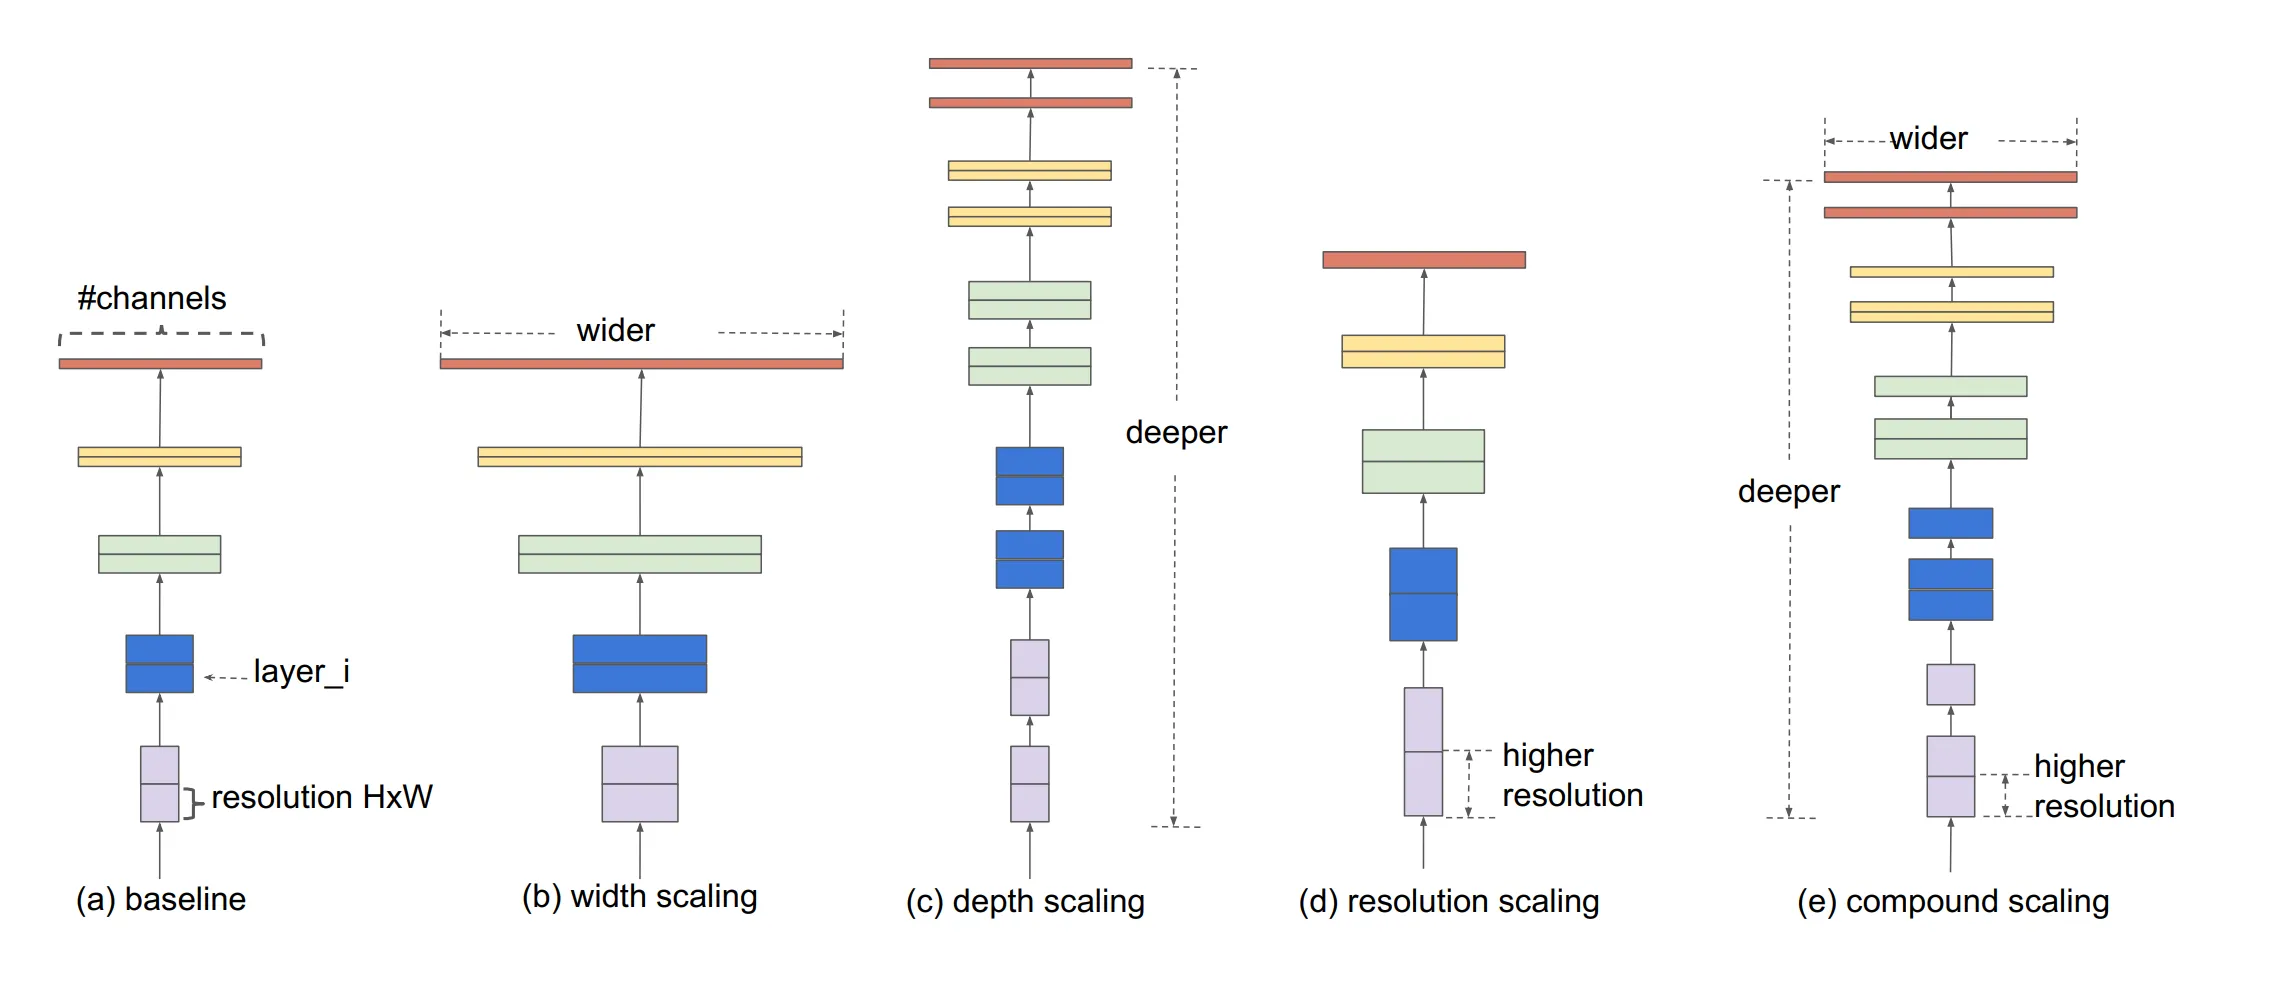
\includegraphics[width=1.05\linewidth]{images/cnn/ENet_1.png}
        \caption*{EfficientNet Scaling.}
    \end{figure}

\framebreak

    \begin{itemize}
        \item \textbf{Compound Scaling} Uses a single \textbf{scaling coefficient} (\(\phi\)) to control:
        \begin{itemize}
        \item \textbf{Network Depth} (\(\alpha^\phi\)) → More layers
        \item \textbf{Network Width} (\(\beta^\phi\)) → More channels per layer
        \item \textbf{Input Resolution} (\(\gamma^\phi\)) → Larger input images
    \end{itemize}
        \item The goal: find \(\alpha, \beta, \gamma\) that balance accuracy \& efficiency, then scale up optimally by increasing the global coefficient \(\phi\).
    \end{itemize}

\framebreak

    \begin{itemize}
        \item EfficientNet optimizes depth, width, and resolution using this constraint:
        \[
        \alpha \cdot \beta^2 \cdot \gamma^2 \approx 2
        \]
        \item \textbf{Why this equation?}
        \begin{itemize}
            \item Increasing \textbf{depth} (\(\alpha\)) increases FLOPs \textbf{linearly}.
            \item Increasing \textbf{width} (\(\beta\)) increases FLOPs \textbf{quadratically} (\(\beta^2\)).
            \item Increasing \textbf{resolution} (\(\gamma\)) increases FLOPs \textbf{quadratically} (\(\gamma^2\)).
        \end{itemize}
        \item To double total FLOPs, the three factors must be balanced together.
    \end{itemize}

\framebreak

    \begin{itemize}
        \item The authors of EfficientNet searched for the best scaling factors on a small baseline model.
        \item They found:
        \[
        \alpha = 1.2, \quad \beta = 1.1, \quad \gamma = 1.15
        \]
    \end{itemize}
\end{frame}

\begin{frame}{EfficientNet Scaling: B0 to B7}
    \begin{itemize}
        \item The EfficientNet family (B0 to B7) is generated using:
        \[
        \text{Depth} = 1.2^\phi, \quad
        \text{Width} = 1.1^\phi, \quad
        \text{Resolution} = 1.15^\phi
        \]
    \end{itemize}

    \begin{table}[]
        \centering
        \begin{tabular}{|c|c|c|c|}
            \hline
            \textbf{Model} & \(\phi\) & \textbf{Depth} (\(\alpha^\phi\)) & \textbf{Width} (\(\beta^\phi\)) \\ 
            \hline
            B0 & 0 & \(1.2^0 = 1.0\) & \(1.1^0 = 1.0\)  \\ 
            B1 & 1 & \(1.2^1 = 1.2\) & \(1.1^1 = 1.1\)  \\ 
            B2 & 2 & \(1.2^2 = 1.44\) & \(1.1^2 = 1.21\)  \\ 
            B3 & 3 & \(1.2^3 = 1.73\) & \(1.1^3 = 1.33\)  \\ 
            B4 & 4 & \(1.2^4 = 2.07\) & \(1.1^4 = 1.46\)  \\ 
            B5 & 5 & \(1.2^5 = 2.49\) & \(1.1^5 = 1.61\)  \\ 
            B6 & 6 & \(1.2^6 = 2.99\) & \(1.1^6 = 1.77\)  \\ 
            B7 & 7 & \(1.2^7 = 3.58\) & \(1.1^7 = 1.94\)  \\ 
            \hline
        \end{tabular}
        \caption*{Scaling EfficientNet from B0 to B7}
    \end{table}

    \begin{itemize}
        \item We multiply these scaling factors by the baseline EfficientNet-B0 values and round to the nearest integer to get the new depth, width, and resolution for each model.
    \end{itemize}
\end{frame}


\begin{frame}{EfficientNet}
    \begin{itemize}
        \item EfficientNet models achieve state-of-the-art accuracy with significantly fewer parameters and FLOPs.        
        \pause
        \item EfficientNet-B7 reaches 84.4\% Top-1 and 97.3\% Top-5 accuracy on ImageNet.
        \pause
        \item More efficient than previous CNN models---8.4x smaller and 6.1x faster than competitors.
    \end{itemize}
\end{frame}


\begin{frame}{EfficientNet Performance}
    \begin{figure}
        \centering
        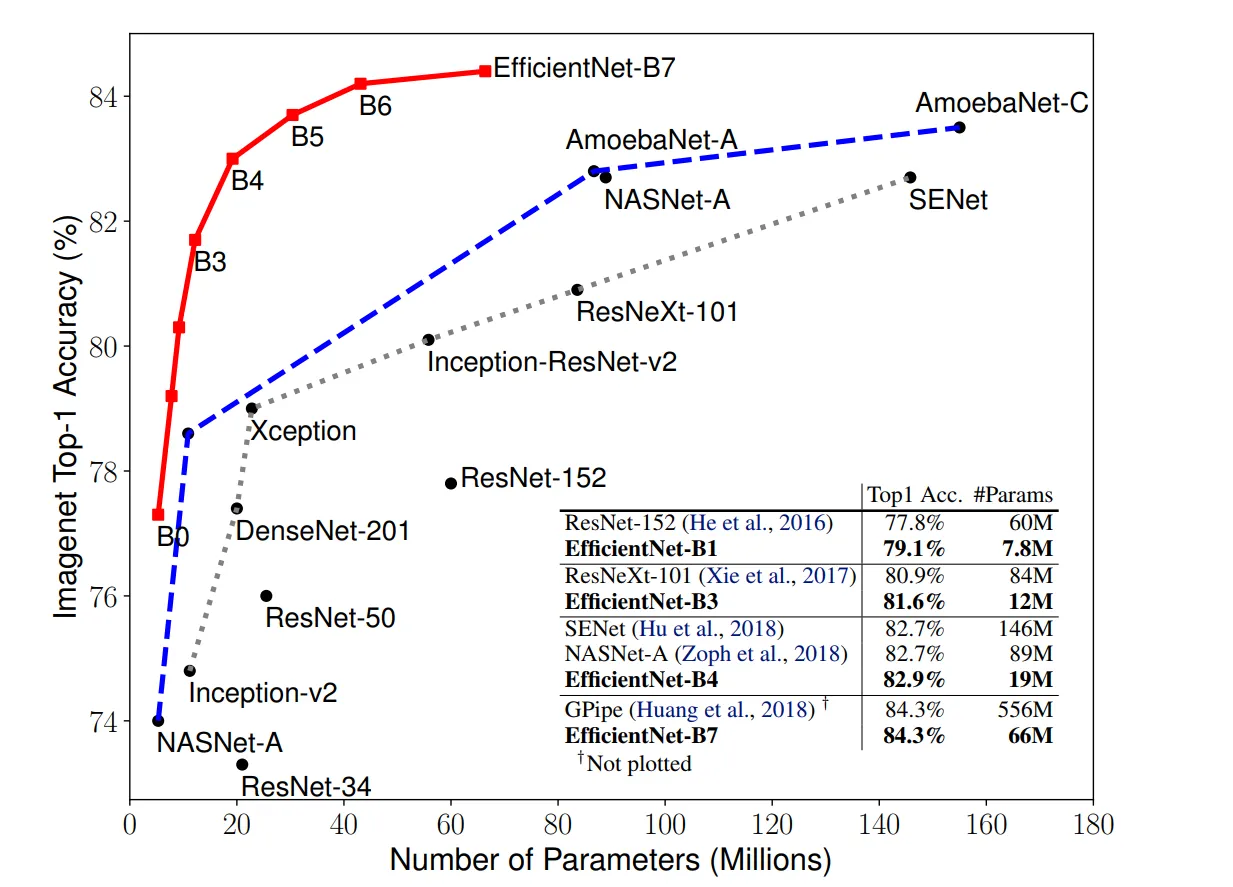
\includegraphics[width=\textwidth,height=.7\textheight,keepaspectratio]{images/cnn/ENet_2.png}
        \caption*{EfficientNet Performance on Imagenet.}
    \end{figure}
\end{frame}
